\newpage
\section{Architecture design and technical decisions}
% ------------------------------------------------------------------------------------------------
\subsection{Parsing grammar (ADP)}
{\color{red}
Borrowing from ADP XXX

XXX: explain ADP concepts

restriction from ADP: we give only the best answer, do we care about semi-optimal ones? no

XXX: normalization, transforms applied

XXX: Think how to implement {\tt cyclic} problems and {\tt windowing} properties within the language

\begin{verbatim}
restrict to only 1 max/min (more restrictive than ADP)
for optimization we want to split grammar into binary productions, to do that we need
to have equality on the following formula. We can solve it more easily if functions are linear
\end{verbatim}
\[\min\limits_{i<k_1<k_2<j}\big[ f(i,k_1,k_2,j) \big] \le  \min\limits_{i<k_2<j} \big[ g_2(i,\min\limits_{i<k_1<k_2} \big[ (g_1(i,k_1,k_2  ) \big],k_2,j) \big]  \]

}

\subsection{Backtracking}
In order to do a clean and efficient transformation from ADP-like language to plain C recurrences, we need to construct bottom-up recurrences from top-down parser rules. To do that, we slightly need to modify the ADP language in order to separate the backtracking and the scoring, because we want to obtain an efficient algorithm: backtrack reads are in $O(n^2)$ whereas score reads are proportional to the algorithmic complexity ($O(n^3)$ or more for non-serial). To deal with this problem, we are facing two options:\ul
\item \textbf{Explicit backtracking:} requires clear syntactical separation between the score and the backtrack and is not implemented in vanilla ADP (unless the whole backtrack is made part of the scoring: big performance impact and non-constant memory requirement issues make its GPU implementation hard and not desirable). Since the backtracking is user-defined, there is no way to generate the backtracking algorithm automatically, hence the user also needs to provide it. 

\item \textbf{Implicit backtracking:} implies that every rule needs to be normalized, and transformed such that given a rule identifier and a set of indices (subproblems breaking), it is possible to retrieve the subproblems combination that build the problem. To do that we need to apply the following transformations\ol
	\item Normalize rules and identify them uniquely by \ul
		\item Removing all the <<or>> operators by breaking a parser into multiple subrules
		\item Forwarding names: replace a rule that is a single invocation by its content (i.e. name a terminal parser with its own name instead of its containing parser's)
		\item Assigning each subrule an unique identifier $r$ and create a mapping table $T: r \to$ user-defined name of the parser.
	\ule
	\item The data elements corresponding to a rule are (scoring, backtracking) and named after the tabulation. The scoring is a user-defined primary type (int, double, ...) and the backtracking is a tuple $({\rm id}_{\rm subrule}, k_1, k_2, \ldots , k_m)$ where $m$ is the maximal number of splits that can occur in the subrules.
	\item During the matrix computation of cell $(i,j)$, if the subrule $r$ applies, the backtrack will be set as $(r,k_1,k_2,\ldots,k_{m_r})$ (obviously with $i\le k_1\le k_2\le \ldots k_{m_r}\le j$ and $m_r\le m$).
	\item During backtracking, when reading the cell $(i,j)$ with backtrack $(r,k_1,k_2,\ldots,k_m)$, given $r$, we recover the subrule hence the user-defined name of the rule that applies and $k_{m_r}$, which allows us to enqueue the subwords $(i,k_1), (k_1,k_2), ..., (k_{m_r})$ for further backtracking. If $r$ refers to a terminal, we stop the backtracking.
	\item The backtracking can be returned to the user as a mapping table $T$ and a list of triplets $(r,i,j)$ where $r$ is the index of the sub-rule that can be easily mapped into the user name (such that $T: r_u \to$ user-defined rule name) and $(i,j)$ is the subword on which the rules applies.
\ole
In short, we break parsers into normalized rules, the backtracking information is the rule id (which rule to unfold) and a list of indices (how to unfold it).
\ule
Assuming that the backtracking information is meant to guide further processing, we provide this information into a list constructed bottom-up: it can be simply processed by the user program in-order, applying for each user-defined rule the underlying transformation, and storing intermediate results (i.e. in a hash map) until they are processed by another rule. Since consumed sub-result can be dropped and since the backtracking contains only relevant sub-problems, ultimately, only the result will be stored.

% ------------------------------------------------------------------------------------------------
\subsection{Memory management}
We denote by \textit{device} the computational device on which the processing of the DP matrix (or of a computational block) is done and $M_D$ its memory. This can be the GPU or the FPGA internal memory. Usually the main memory is larger than device memory and can ultimately be extended by either disk or network storage.

We propose to evaluate the device memory requirements to solve the above problem classes. We need first to define additional problem properties related to implementation:\ul
\item \textbf{Number of matrices:} multiple matrices can be encoded as 1 matrix with multiple values per cell. Hence the implementation differentiates only between cost and backtrack matrices with respective element sizes $S_C$ and $S_B$.
\item \textbf{Delay of dependencies:} In case the problem does not fit into memory, partial matrix content needs to be transferred across sub-problems. Such data amount is usually proportional to the delay of dependencies. If this delay is small, it might be worth to duplicate matrix data in the wavefront, otherwise it might be more efficient to allow access to the previous computational blocks of the matrix.
\item \textbf{Wavefront size:} Finally some aggregation that is made along some dimension of the matrix does not need to be written at every cell but can be propagated and aggregated along with computation (ex: maximum along one row or column). Hence such information can be maintained in a single place (in the wavefront) and progress together with the computation. We denote by $S_W$ the size of wavefront elements.
\item \textbf{Input size:} the size of an input letter (from input alphabet) is denoted by $S_I$.
\ule

% ----------------------------------------------
\subsubsection{Small problems (in-memory)}
Problem that can fit in memory can be solved in a single pass on the device. Such problem must satisfy the equation:
	\[(S_I+S_W) \cdot (m+n) + (S_C+S_B) \cdot (m\cdot n) \le M_D\]

For instance, assuming that $m=n$, $M_D=1024{\rm Mb}$, that backtrack is 2b (<16384, 3 directions) and that the cost can be represented on 4 b (int or float), that input is 1b (char) and that there is no wavefront, we can treat problems of size $n$ such that $2n+5n^2 \le 2^{30} \implies  n\le 14650$. We might also possibly need to take into account extra padding memory used for coalesced accesses. But it is reasonable to estimate that problems up to 14K fit in memory.

% ----------------------------------------------
\subsubsection{Large problems}
To handle large problems, we need to split the matrix into blocks of size $B_H \times B_W$. For simplification, we assume a square matrix made of square blocks with $b$ blocks per row/column.

% ----------------------------------------------
\subsubsection{Non-serial problems}
Non-serial problems need to potentially access all elements that have been previously computed. We restrict\footnote{As we have not encountered a problem with non-serial dependencies along the diagonal.} ourselves to the following dependencies: \ul
\item Non-serial dependencies along row and column
\item Serial dependencies along diagonal, with delay smaller or equal to one block size
\ule
Such restriction implies that all the block of the line and the row, and one additional block to cover diagonal dependencies must be held in memory (independently of the matrix shape).

For simplification, let $m=n$ and assume that we have $b$ square blocks per row and per column. Hence we have the following memory restriction:
\[ 2\frac{n}{b}(S_I+S_W) + 2 \cdot \frac{n^2}{b}S_C + \frac{n^2}{b^2} S_B \le M_D\]

We also need to take into account the transfer between main memory (or disk) and device memory. Dependency blocks only need to be read, computed blocks need to be written back. Ignoring the backtrack and focusing only on the cost blocks, the transfers (in blocks) are:
\[\begin{array}{rclll}
		b^2 +% computed line writeback (once)
		(b-1)^2 + % diagonal block loads (1 per block)
		\sum\limits_{i=0}^{b-1} i \cdot b % column dependencies loads (for line i)
		&=&\tfrac{1}{2}b^3+\tfrac{3}{2}b^2-2b+1 &\qquad& \rm (Rectangle)
	\\
		\sum\limits_{i=1}^{b} \Big(1+2\cdot(i-1)\Big) \cdot (b+1-i) % on i_th diagonal
		&=& \tfrac{1}{3} b^3 + \tfrac{1}{2}b^2 + \tfrac{1}{6}b &\qquad& \rm (Triangle)
	\\
		\sum\limits_{i=1}^{b} \Big(1+2\cdot(i-1)\Big) \cdot b % on i_th diagonal
		&=& b^3 &\qquad& \rm (Parallelogram)
\end{array}\]

Putting these two formula together, and using most of the device memory available, we obtain the following results with $S_C=4, S_B\footnote{To deal with larger matrices, backtrack data need to be extended.}=4, S_I=1, S_W=0$ and $M_D=2^{30}$:
\begin{center}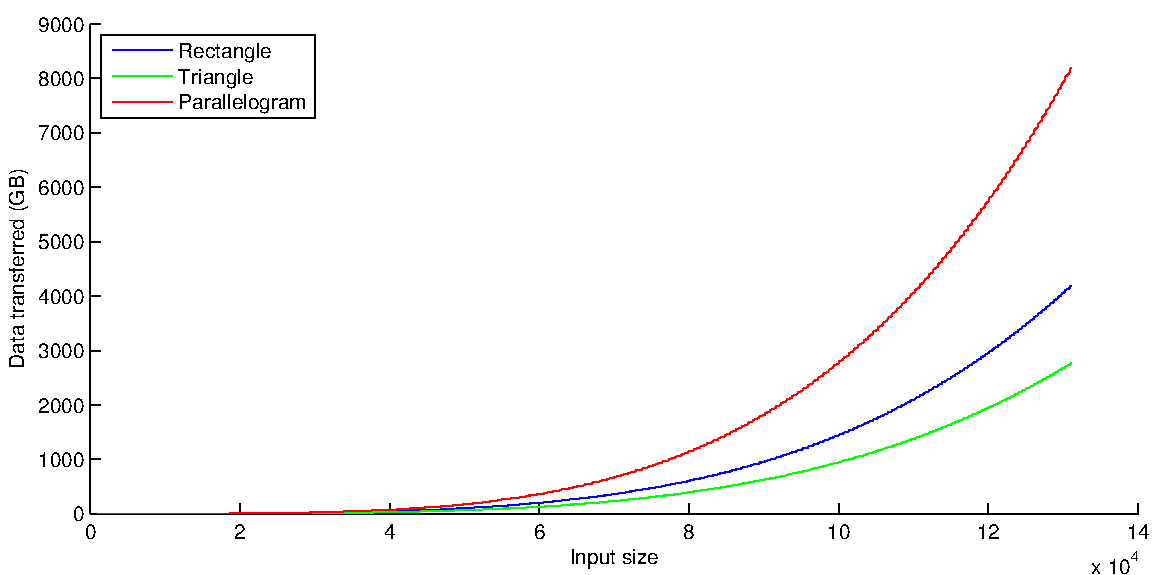
\includegraphics[width=14cm]{inc/ns_large.pdf}\end{center}

Given an experimental bandwidth of 5.3743 Gb/s between CPU and GPU, processing matrices one order of magnitude larger (128K) would result in respectively 13\up{(R)}, 8.5\up{(T)} and 25.4\up{(P)} minutes of transfer delay. Extrapolating the preliminary results of small problems, a computation on input of size 128K would require respectively 7 days 13h\up{(R)}, 2 days 22h\up{(T)} and 6 days 10h\up{(P)}, assuming there is no other scalability issues. Although this overhead seems appealing compared to the computation time, the total time blows up (because of the  $O(n^3)$ complexity) and make the processing of such large problem less relevant. Given that real problems -- like RNA folding -- operate at input sizes up to 4096, it would not be of much relevancy to implement a version for larger cases, although perfectly feasible.

% ----------------------------------------------
\subsubsection{Serial problems}
The serial problem have the interesting property to access to a fixed number of previous elements. These elements can be either stored either explicitly in a scoring matrix or implicitly as moving aggregation into a wavefront. Since the dependencies are fixed, the computation direction gains an additional degree of freedom: matrix can be solved in diagonal (as non-serial problems) or line-wise or column-wiser. This allows to store the whole necessary state to make progress into a limited number of lines (or columns), and sweep vertically (resp. horizontally) along the matrix.

Since serial problems are of complexity $O(n^2)$ (due to the matrix dimension and the finite number of dependencies), it is possible to tackle much larger problem than non-serial during the same running time. Hence, it seems obvious to let serial problems grow larger than the memory.

Mixing the dependency property and size requirements, we can split the matrix into sub-matrices, store special lines (and/or columns) into memory (or hard disk), and repeat computations to solve the backtrack (similarly as in \cite{swat_gpu},\cite{swat_mega}, but this implementation use problem-specific knowledge that might not generalize).

To store intermediate lines and columns, we are facing two different strategies to explore:\ul
\item \textbf{Fixed subproblem size:} we decompose the algorithm as follows\ol
\item Define a grid of <<major column and rows>>, where each cell's data (input, output, cost and backtrack matrices) fits into the device memory.
\item Compute the values of the grid's major columns and rows in one pass.
\item Second (on-demand) computation to process backtracking inside relevant cells.
\ole
Let $b$ the number of cells that we have on each row/column, the total computation running time would be $(b^2 + 2b) \cdot t_b$ where $t_b$ is the time to compute one cell's matrix. This division has the advantage of providing the minimal computation time at the expense of external storage proportional to $O(n)$ (if we store only lines or columns) or $O(n^2)$ (if we store both).

\item \textbf{Myers and Miller’s algorithm:} (divide and conquer)
This algorithm break the DP problem into 2 (or 4) subproblems such that once the middle line/column is computed, the problem can be solved for 1 submatrix and backtracking among up to 2 of the 3 other. This breaking is applied recursively until the submatrix data fits into memory. The storage requirements are $4 \cdot O(n)$ (we store along both dimension $1+\tfrac{1}{2}+\tfrac{1}{4}+...$ lines/columns).

The algorithm proceeds as follows: first it solves the problem to obtain the first backtracking element, then it breaks the matrix in 4 submatrices, and refine it until backtrack is tractable. Since there is at most $\log n/b$ refinements and since every part of the matrix may be involved in backtrack, running time is $O(n^2 \log_2 n)$.
\item \textbf{Hybrid approach:} a hybrid approach might be created to take advantage of additional available memory, however, the running time decreases logarithmically to the space used.
\ule

{\color{red}
try to setup wavefront size (if needed) => just enlarge the matrix by 1 so that we go wavefront-to-wavefront

XXX: what's the maximal size of the wavefront ??

XXX: can we avoid to store some matrices and put them in the wavefront ??

Split into blocks:\ul
\item Decide the shape of the blocks
\item Decide the size of the blocks
\item Decide of a strategy to store intermediate lines/columns: space/time tradeoff.
\ule

XXX: make it work up to 14K for all 3 problems using multiple kernels
XXX: example of non-symmetric serial problem

The three last elements, combined with the above one, provide a precise estimation of the memory consumption, and the implementation difficulty 

all the problem are subject to the input dimensions $n$.

the two latter one gives an estimation of the constant factor.

The delay of dependencies might also have an impact: if the matrix is too large to fit in the memory (device or main memory), it becomes necessary to maintain partial matrix content (all the intermediate elements) within the wavefront. Also the number of cost matrices might affect the performance, simply because maintaining them requires computations and memory accesses.
}

% ------------------------------------------------------------------------------------------------
\subsection{Memory layout}


% ------------------------------------------------------------------------------------------------
\newpage
\subsection{LMS compiler stack}
\textbf{User-language}: define additional parameters for the recurrence\ul
\item Windowing (to convert non-serial into serial problems)
\item Input sizes, and alphabets (backtrack, input, cost)
\item Backtrack (implicitly by backtrack alphabet size) and cost matrices bit-sizes (cost maximum may be inferred using <<Yield size/grammar analysis>>)
\item Recurrence functions, devices available
\item What to keep in memory (cost, backtrack or both).
\ule
$\Downarrow$ Conversion (using an existing technique)

\textbf{Intermediate representation}

$\Downarrow$ Optimizations\ul
\item Transform non-serial into serial \ul
	\item Use aggregation functions/transformations
	\item Use windowing from user (if no other technique succeed)
	\ule
\item Define the wavefront depth
\item Avoiding the cost matrix by moving it into the wavefront
\ule

\textbf{Code specification}\ul
\item Kernel function (1-element function), inputs, outputs, wave front, dependencies, bit sizes
\item Device-level interface => setup the block sizes(w/h), input and memory sizes
\item Define the device-specific implementation of the block (CPU/FPGA/CUDA)
\item Define the co-processor memory aggregation function
\item Define the scheduling of the blocks and aggregation (software pipelining)
\item Define the data movement back and forth to disk
\ule

$\Downarrow$ Generation\ul
\item Generate the kernel for specific device
\item Generate the scheduling and barriers
\ule

\textbf{Binary program}

%\ol
%\item Make sure we encompass all the most common patterns of DP: check if we have higher dimensions or more complex formula.
%\item Let the user tune the window size if he wants to reduce non-serial to serial.
%\item Concerns separation: common architecture enables flexibility (exchange components) \ul
%	\item Block processor: CPU, GPU, FPGA, must allow variation of width and height
%	\item Memory stats computation (min, sum, ... column/line combinations): CPU, GPU
%	\item Scheduler (CPU): interleave block computation and memory statistics
%	\ule
%\item Common description \ul
%	\item Block kernel processor
%	\item Full block
%	\ule
%\item Discussion: wavefront, design similarities, polyhedral theory
%\ole

%%\newcolumntype{C}[1]{>{\centering\let\newline\\\arraybackslash}m{#1}}
%\newcolumntype{C}{@{\hspace{7pt}}c@{\hspace{7pt}}}
%\def\mnl{\rule{0pt}{2.6ex}\rule[-1.2ex]{0pt}{0pt} \\ \hline}
%$\begin{array}{|C|C|C|C|C|C|} \hline
%0 & 0 & 0 & 0 & 0 & 0 \mnl
%0 &  &  &  &  & \mnl
%0 & M_{23}  &  &  &  & \mnl
%0 &  & \sum  &  &  & \mnl
%0 &  &  &  &  & \mnl
%0 &  &  &  &  & \mnl
%\end{array}$
%\end{document}
